\chapter{Simulation study}
After developing FHTBoost (see chapter \ref{ch:FHTboost}), we wish to verify that it works, i.e. that it has predictive power and selects correct variables.
Not only that, but we wish to see which of the two versions of the algorithm works best, namely the fixed intercept version and the version with an iteratively changing intercept.

One way to verify that a statistical estimation method works, is to test it on simulated data.
Simulation studies are used for many different purposes, but a particularly common purpose is to simulate survival data from the ``true model'' (in this case, our first-hitting-time model), for which we know the true values of the parameters.
We can then use our developed method to estimate these parameters, and see how well it recovers the true parameters in the final model, and how well the model fits the simulated data.
The model should fit the simulated data well, because the data generating mechanism \textit{is} the model.

In addition to verifying that the algorithm works, 
The fixed intercept version or the changing intercept version.


\section{Simulation design}
In this chapter we describe two scenarios, a highly correlated scenario and an uncorrelated scenario. 
The purpose of each scenario is to estimate FHT parameters, using the FHTBoost algorithm, on data simulated according to the scenario, and then to assess the model's performance on this data.
In both scenarios, we generate a high-dimensional covariate matrix $\X$ consisting of covariate vectors
\begin{equation}
    \x_1,\x_2,\ldots,\x_{p_1},
\end{equation}
which is supposed to mimic gene expression data.
We also have a low-dimensional covariate matrix $\Z$, which similarly consist of covariate vectors
\begin{equation}
    \z_1,\z_2,\ldots,\z_{p_2},
\end{equation}
and which is supposed to mimic clinical measurements.
We link each covariate to a parameter in a parameter vector, where $\X$ corresponds to $\bbeta$, and $\Z$ corresponds to $\bgamma$.
In each parameter vector, $\bbeta$ and $\bgamma$, we set only a small number of parameters to a non-zero value, and we set all the rest to zero.
Thus only a very small number of covariates will have an effect.
Given these parameter vectors and covariate matrices, we can calculate a specific $y_{0,i}$ and a specific $\mu_i$ for each individual $i$, $i=1,2,\ldots,N$, where $N$ is the size of the data set.
From the FHT perspective, discussed previously in section \ref{fht-idea} and onward, these are parameters which represent the health process of each individual.
To reiterate, an individual $i$ has a stochastic health process, a Wiener process, with an initial level $y_{0,i}$ and a drift $\mu_i$.
Consequently its lifetime follows the lifetime probability distribution $\IG(y_{0,i},\mu_i)$.
This relationship allows us to easily draw a lifetime for each individual from its respective inverse Gaussian distribution.

It is important to evaluate the model/algorithm performance (both in terms of predictive ability and variable selection) on a separate and unseen test set.
Each training set will be generated by drawing $N=500$ individuals as described above, with a specific seed.
Since we are simulating, it is simple to generate a test set by drawing from a unique seed.
We are therefore also able to decide the size of the test set.
We set $N_{\text{test}}=1000$ observations.

We generate $B\approx500$ data sets by drawing survival data according to algorithm \ref{algo:clinical-sim}, such that each data set has $N=500$ observations. 
We treat each data set as a separate training data set, and thus estimate $B$ models.
To estimate each model, we first a perform repeated 5-fold cross validation procedure (see subsection \ref{subsec:K-fold}), with 5 repeats, on the training data set.
As shown in subsection \ref{subsec:iterations}, this should provide a reasonably variance reduced estimate of $\mstop$ (near the ``true'' $\mstop$).
We then estimate a model on the training set, by running FHTBoost with $\mstop$ number of iterations.

The boosting algorithm has two main purposes: Selection of variables, and minimizing test error.
To assess variable selection, we look at some well known metrics.
To assess the test/generalization error, we finally calculate the difference of deviance on the test set.

\section{Simulation of survival data from an IG FHT distribution}\label{sec:simulate-IG-data}
We wish to simulate survival times $\ti,i=1,\ldots,n$ with censoring.
We first draw $n$ (uncensored) survival times $\{\tilde{t}_i\}_{i=1}^n$ from a survival time distribution $f(\cdot)$.
If this distribution has a closed form probability distribution function, we can draw from it directly.

To censor the data, we draw censoring times $w_i\sim f(\cdot),i=1,\ldots,N$ from some other lifetime distribution where the parameters do \textit{not} depend on covariates.
We let the observed survival times then be $t_i=\min(\tilde{t}_i,w_i)$.
The corresponding censoring indicator, $d_i$, is then set equal to 1 if the actual survival time was observed, i.e., if $\ti<w_i$.
We end up with a set of $N$ tuples $(t_i,d_i),i=1,\ldots,N$.
Note that this prcedure simulates censored time under independent censoring, since indeed the censoring times are independent of the survival times.

\begin{algorithm}
\caption{Generating survival data from Inverse Gaussian FHT distribution}
\label{algo:FHT-sim}
\begin{enumerate}
    \item Obtain the design matrices $\X$, $\Z$ and the true parameter vectors $\bbeta$ and $\bgamma$.
    \item\label{algo:FHT-sim-step-cens} Specify a censoring time distribution.
    \item Calculate the distribution parameters $y_0$ and $\mu$ using the link functions,
        \begin{align*}
            y_0&=\exp(\bbeta^T\X)=\exp\left(\beta_0+\sum_{j=1}^p\beta_jx_j\right), \\
            \mu&=\bgamma^T\Z=\gamma_0+\sum{j=1}^d\gamma_jz_j.
        \end{align*}
    \item Draw $N$ uncensored survival times $(\tilde{t}_i)_{i=1}^N$ from IG$(\mu,y_0)$.
    \item Draw $N$ censoring times $(w_i)_{i=1}^N$ from the censoring time distribution specified in step \ref{algo:FHT-sim-step-cens}.
    \item Right censor the survival times by choosing
            \begin{equation*}
                t_i=\min(\tilde{t}_i,w_i).
            \end{equation*}
          The censoring indicator on whether observation $i$ was observed or not is then
          \begin{equation*}
            d_i=I(t_i=\tilde{t}_i).
          \end{equation*}
    \item The simulated data set is $D=(t_i,\,d_i)_{i=1}^N$.
\end{enumerate}
\end{algorithm}

\section{Generating correlated clinical and gene expression data}
To create a realistic scenario where we have data looking like gene expression data and clinical data, we need to define a proper correlation structure.
We can draw covariate matrices from a normal distribution with a suitable covariance matrix.

We consider a scenario where we have a covariate matrix $X$ consisting of $p$ gene expressions, and a covariate matrix $Z$ consisting of $d$ clinical measurements.
We can imagine that some of the genes in $X$ are highly correlated.
One way to imagine this is to imagine that we have blocks of genes,
where inside one block, the genes are highly correlated, whereas genes in one block are not correlated to other genes.
In addition, one block of genes might affect a block of clinical variables as well.

We specify a number of blocks $B$. A given block $b,b=1,2,\ldots,B$, contains a certain number of genes, $G_b$, which are correlated to each other.
It also contains a certain number of clinical measurements, $C_b$. These measurements are correlated to each other, and to the genes in the block.

After setting up the block structure, we 
\todo[inline]{Finish this}

There are three types of correlations.
1. Within each block of genes. Defaults to 0 for genes not belonging to any block.
2. Between clinical predictors in each pathway
3. Between the clinical and molecular predictors in each pathway

Algorithm \ref{algo:clinical-sim} contains a schematic overview.


\section{General simulation procedure}
We perform simulations in which the observations are drawn from the inverse Gaussian distribution, i.e., we simulate lifetimes from the first hitting time model with Wiener process as the health process.
We do this by using algorithm \ref{algo:FHT-sim}.
We will have two scenarios:
(i) No correlation, and (ii) correlation.
To simulate the covariate matrices $X$ and $Z$ we will use Algorithm \ref{algo:clinical-sim}, which is a method for simulating clinical and gene data together.
We imagine $X$, corresponding with regression parameter vector $\bbeta$, be gene expressions, whereas $Z$, which is corresponding to the vector of regression coefficients $\bgamma$, be clinical measurements.
We specify the different correlations for the covariate matrices.
But most importantly, we specify the true parameter vectors, $\bbeta$ and $\bgamma$.
For each scenario, we conduct $N_{\text{scenario}}$ runs.

One run consists of first drawing data (with a specific seed to ensure reproducibility), i.e., we draw covariate matrices $\X$, $\Z$ from Algorithm \ref{algo:clinical-sim}.
$\X$ is of size $n\times p$ and $\Z$ is of size $n\times d$, where $n$ is the number of observations, $p+1$ is the size of the covariate vector $\bbeta$ (including an intercept which will not be affected by the covariates), and $d+1$ is the size of the covariate vector $\bgamma$.
Then we combine these with the true covariate matrices to get vectors $\y_0$ and $\mathbf{\mu}$ of initial value of the health process, and drift, respectively.
Then we draw from the Inverse Gaussian distribution according to Algorithm \ref{algo:FHT-sim}, obtaining $N$ right-censored lifetimes, i.e., $n$ tuples $(t_i,d_i)_{i=1,\ldots,N}$.
With these tuples, then, we can do a run with the FHT boosting algorithm. We first use repeated K-fold cross-validation to find the optimal number of boosting steps, $m_{\text{stop}}$.
Then we estimate the model on the whole of this training set.
Then we validate this model on a test set of size $N_{\text{test}}$.
The data here are drawn in the exact same manner as the training data, again with a specific seed for reproducibility.

\begin{algorithm}
\caption{Generating correlated clinical and gene expression data}
\label{algo:clinical-sim}
\begin{enumerate}
    \item Lorem ipsum.
\end{enumerate}
\end{algorithm}

\section{Scenarios}
\subsection{Scenario 1: Uncorrelated case}

Here, $N$ is 500. We let $\bbeta$ be a large vector of size $p=10001$, and $\bgamma$ be a small vector of size $d=16$. Specifically, we set the intercept term in $\bbeta$ to be 2.0, and the first 35 elements to be 0.1. We set the rest to be 0. For $\bgamma$, we set the intercept term to be -1, and in similar fashion, let the first 5 elements have a non-zero value of -0.1. Here also we set the remaining 10 elements to be 0.
Hence, the true parameter vectors are as follows:
\begin{align*}
    \bbeta=\left(2.0, \underbrace{0.1, 0.1, \ldots, 0.1}_{\text{length 35}}, \overbrace{0, 0, \ldots, 0}^{\text{length 9965}}\right) \\
    \bgamma=\left(-1.0, \underbrace{0.1, 0.1, \ldots, 0.1}_{\text{length 5}}, \overbrace{0, 0, \ldots, 0}^{\text{length 10}}\right)
\end{align*}
We draw $X$ and $Z$ from Algorithm \ref{algo:clinical-sim} for drawing clinical and gene data, with $B=0$ blocks.

Choosing 0.1 for the informative parameter effects $\beta_j,j=1,2,\ldots,35$, might seem like it is too low.
The parameter vector $\bbeta$ is linked to the initial level $y_0$ by an exponential link function, as usual.
This means that each parameter effect is multiplicative instead of additive.
A large gene expression value here can potentially cause a large change in $y_0$, and especially if there are several rather extreme values, due to the multiplicative effect.
With 35 genes that do affect $y_0$, the chance of having one or several large gene values is rather large.
Although we do standardize before drawing.
Because of this, I had trouble setting up any simulation in which the algorithm managed to pick up much of the underlying parameter vector.
The reason the parameter sizes on the drift are so small is that the effect is linear with time.
We specify that all correlations are 0, meaning no covariate correlates with any other.

With this exact setup, we run a simulation experiment $B=500$ times, where we set the seed at the beginning of each simulation.
We first generate matrices $X$ and $Z$ from Algorithm \ref{algo:clinical-sim}, with all correlations set to 0.
Based on these covariate matrices, we simulate FHT lifetimes from Algorithm \ref{algo:FHT-sim}.
Having now a data set $D_b$, we run cross validation on this data set to find the optimal iteration number $m_{\text{stop}}$.
See Figure \ref{fig:simulation-uncorrelated-deviances-boxplot}
We then run a boosting algorithm with $m_{\text{stop}}$ steps on the training set, to estimate parameters.


Finally, we calculate the deviance of the estimated model on the test set.

\subsection{Scenario 2: Correlated}
Consider now a scenario where we have correlation in different ways.
We have blocks of genes which are correlated, meaning the genes comprising one are correlated.
Further, the genes in a block of genes are correlated with certain clinical measurements.
Finally, the clinical measurements are correlated.
All these correlations are set to 0.7.
In other words, this is a scenario with highly correlated data.

There are three types of correlations.
1. Within each block of genes. Defaults to 0 for genes not belonging to any block.
2. Between clinical predictors in each pathway
3. Between the clinical and molecular predictors in each pathway

\section{Results}
\subsection{Uncorrelated case}

\begin{table}
\caption{Difference of deviance results for FHTBoost, uncorrelated case}
\label{table:uncorrelated-deviance}
\centering
\begin{tabular}{l|rr}
\toprule
& Updating & Fixed \\
\hline
Mean               &  -92.0  & -130.1  \\
Standard deviation &   41.8  &   40.7  \\
Minimum            & -233.6  & -255.2  \\
Maximum            &    7.2  &   -5.7  \\
\bottomrule
\end{tabular}
\end{table}

\begin{table}
\caption{High dimensional (genomic) part: Performance of FHTBoost in terms of variable selection, uncorrelated case}
\label{table:uncorrelated-y0}
\centering
\begin{tabular}{l|cc|cc}
\toprule
& \multicolumn{2}{c}{Updating} & \multicolumn{2}{c}{Fixed} \\
& Mean & Standard error & Mean & Standard error \\
\hline
Sensitivity & 0.190 & (0.090) & 0.452 & (0.162) \\
Specificity & 1.000 & (0.000) & 0.997 & (0.002) \\
FDR         & 0.310 & (0.176) & 0.613 & (0.144) \\
\bottomrule
\end{tabular}
\end{table}

\begin{table}
\caption{Low dimensional (clinical) part: Performance of FHTBoost in terms of variable selection, uncorrelated case}
\label{table:uncorrelated-mu}
\centering
\begin{tabular}{l|cc|cc}
\toprule
& \multicolumn{2}{c}{Updating} & \multicolumn{2}{c}{Fixed} \\
& Mean & Standard error & Mean & Standard error \\
\hline
Sensitivity & 0.741 & (0.232) & 0.958 & (0.099) \\
Specificity & 0.943 & (0.110) & 0.638 & (0.291) \\
FDR         & 0.091 & (0.144) & 0.375 & (0.192) \\
\bottomrule
\end{tabular}
\end{table}

\begin{table}
\caption{Optimal iteration number $\mstop$ results for FHTBoost, uncorrelated case}
\label{table:uncorrelated-mstop}
\centering
\begin{tabular}{l|rr}
\toprule
& Updating & Fixed \\
\hline
Mean               &  15.8  &  63.8  \\
Standard deviation &   6.4  &  26.5  \\
Minimum            &     2  &     2  \\
Maximum            &    39  &   160  \\
\bottomrule
\end{tabular}
\end{table}

\begin{figure}
\caption{Boxplot for difference in deviance for the two intercept variants, non-correlated scenario}
\label{fig:simulation-uncorrelated-deviances-boxplot}
\centering
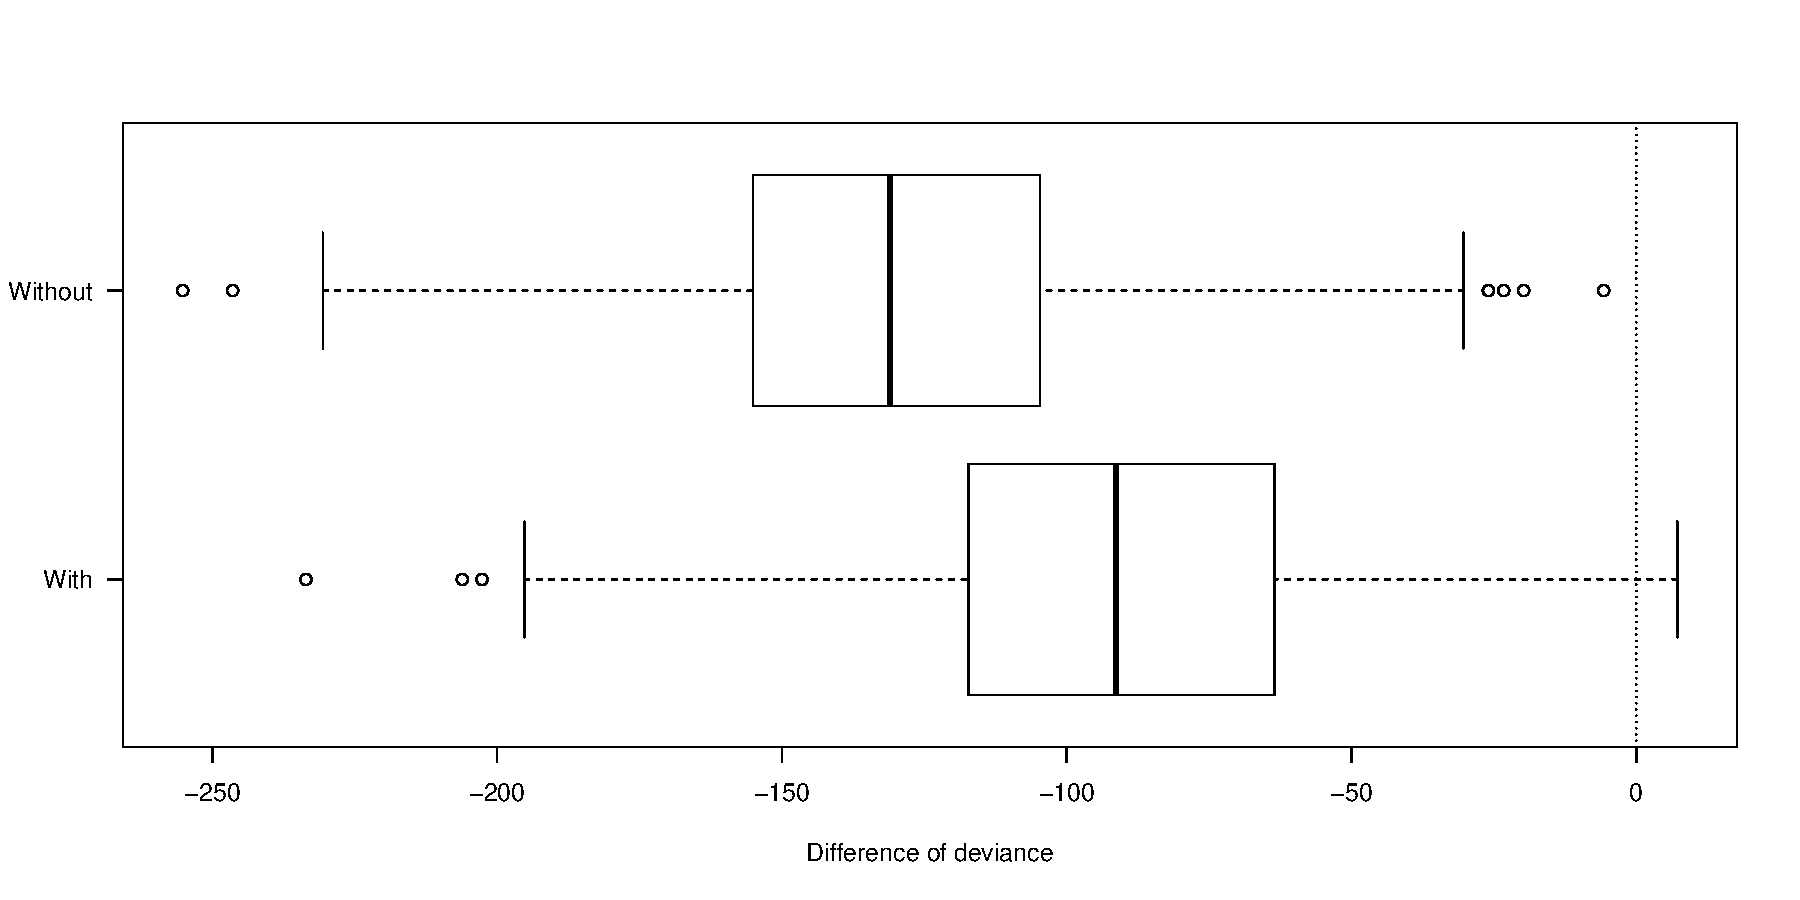
\includegraphics[scale=0.4]{deviances_simulation.pdf}
\end{figure}

The most evident result is that, in contrast to our expectation, the fixed intercept algorithm seems to perform on average better than that with updating intercept.
See Table \ref{table:uncorrelated-deviance}.
Despite the large variability (see min, max and sd in Table \ref{table:uncorrelated-deviance}), this difference is noticeable (see also Figure \ref{fig:simulation-uncorrelated-deviances-boxplot}), especially considering that the fixed intercept version performs always better than the null model, while there are a few cases in which the updating intercept version does not (Table \ref{table:uncorrelated-deviance}, row "min", and Figure \ref{fig:simulation-uncorrelated-deviances-boxplot}).
This can be a consequence of overfitting:
Moving the intercept allows the model to fit the training data too well.


Note first that the two versions of the algorithm have very different $\mstop$ values.
The stopping iteration $\mstop$ when continuously changing the intercept is quite lower than when boosting without.
This means that the resulting covariates for the changing intercept version are more shrunken than for the fixed intercept version.
This suggests that the non-fixed intercept version is quicker to overfit, since the $\mstop$ should find approximately the iteration number which minimizes overfitting.
Since the covariate vector is estimated on the training data, a likely explanation is that the changing intercept captures more of the variation in the training data.
In doing so, there is less variation to be explained by the covariates, and hence the boosting algorithm will start to overfit more quickly.
We see that the median difference of deviance on the updating intercept version is -91.955, while it is -130.109 on the fixed intercept version.
We should therefore conclude that the non-intercept version is better, if we want to choose between the two.
Look at the boxplot in figure \ref{fig:simulation-uncorrelated-deviances-boxplot}.
Another thing to note here is that the fixed intercept version has no occurrence of a positive difference of deviance.
In other words, all estimated models performed better than their null models.

Let us contrast the two versions of FHTBoost in terms of variable selection as well.
In each run, we counted $TP$, the number of informative covariates which were selected in the estimated boosting model.
We similarly counted $TN$, the number of non-informative covariates which were selected in the model.
Our setup has as many as 35 informative gene covariates and 5 informative clinical covariates.
Since the no-intercept version has a rather low number of iterations, with a median of 16, it is usually impossible to get anywhere near perfect on these metrics, as at most one new parameter is selected in each iteration, and we have 40 informative covariates in total from the two vectors.
\todo[inline]{Write this better!}

Furthermore, we are considering the sensitivity and specificity on both covariate vectors at the same time.
This means that these scores will affect each other.

Consider first the result of the version in which the intercept is changed in each step.
Both covariate vectors have a very high specificity, which measures the amount of true negatives which are correctly classified as negatives, i.e., not selected.
In both cases, these are almost 1.
In fact, for $\bbeta$, although it is not exactly 1, but rather 0.999667937538074.
When rounded to 3 significant digits, this is 1, and similarly, the standard error rounded is 0.000.
Keep in mind here that the denominator in these cases is 9965.
If we only look at $FN$, i.e., false positives, which is $N-TN$, the mean is 3.31, with a standard error of 2.50.
With a median false discovery rate of 0.333, there is a one in three chance that we select a variable which is not actually informative.
The sensitivity, i.e., the ratio of correctly selected informative variables, has a mean of only 0.190.
This means that a large proportion of the informative covariates are not selected.
For $\bgamma$, a much higher specificity is attained, with a median at 0.800.
Even though the parameter effects on the drift are rather small, the informative covariates are often correctly selected.
Furthermore, the false discovery rate here is very low, with a median at 0.000.

Now consider the results of the fixed intercept version.
For the $\bbeta$ covariate vector, a higher proportion of informative covariates are selected, with a mean sensitivity of 0.452.
Simultaneously, a larger false discovery rate of 0.584 is not good: This means that more than half should be expected to be false.
At the same time, the $\bgamma$ covariate vector has a really good sensitivity, with a median of 1, and a good specificity with a median of 0.700.
The false discovery rate on $\bgamma$ is slightly above one in three, with a median of 0.375.


\subsection{Correlated case}

\begin{table}
\caption{Difference of deviance results for FHTBoost, uncorrelated case}
\label{table:uncorrelated-deviance}
\centering
\begin{tabular}{l|rr}
\toprule
& Updating & Fixed \\
\hline
Mean               &  -57.8  &  -58.8  \\
Standard deviation &   47.2  &   46.1  \\
Minimum            & -203.4  & -223.1  \\
Maximum            &   87.6  &   73.5  \\
\bottomrule
\end{tabular}
\end{table}

\begin{table}
\caption{High dimensional (genomic) part: Performance of FHTBoost in terms of variable selection, correlated case}
\label{table:correlated-y0}
\centering
\begin{tabular}{l|cc|cc}
\toprule
& Updating & & Fixed & \\
& Mean & Standard error & Mean & Standard error \\
\hline
Sensitivity & 0.157 & (0.084) & 0.204 & (0.081) \\
Specificity & 0.999 & (0.000) & 0.998 & (0.001) \\
FDR         & 0.439 & (0.218) & 0.652 & (0.181) \\
\bottomrule
\end{tabular}
\end{table}

\begin{table}
\caption{Low dimensional (clinical) part: Performance of FHTBoost in terms of variable selection, correlated case}
\label{table:correlated-mu}
\centering
\begin{tabular}{l|cc|cc}
\toprule
& Updating & & Fixed & \\
& Mean & Standard error & Mean & Standard error \\
\hline
Sensitivity & 0.273 & (0.187) & 0.625 & (0.245) \\
Specificity & 0.831 & (0.139) & 0.537 & (0.236) \\
FDR         & 0.454 & (0.250) & 0.507 & (0.130) \\
\bottomrule
\end{tabular}
\end{table}

\begin{table}
\caption{Optimal iteration number $\mstop$ results for FHTBoost, correlated case}
\label{table:correlated-mstop}
\centering
\begin{tabular}{l|rr}
\toprule
& Updating & Fixed \\
\hline
Mean               &  20.0  &  51.1  \\
Standard deviation &  12.1  &  24.4  \\
Minimum            &     2  &     2  \\
Maximum            &    65  &   148  \\
\bottomrule
\end{tabular}
\end{table}

\begin{figure}
\caption{Boxplot for difference in deviance for the two intercept variants, non-correlated scenario}
\label{fig:simulation-correlated-deviances-boxplot}
\centering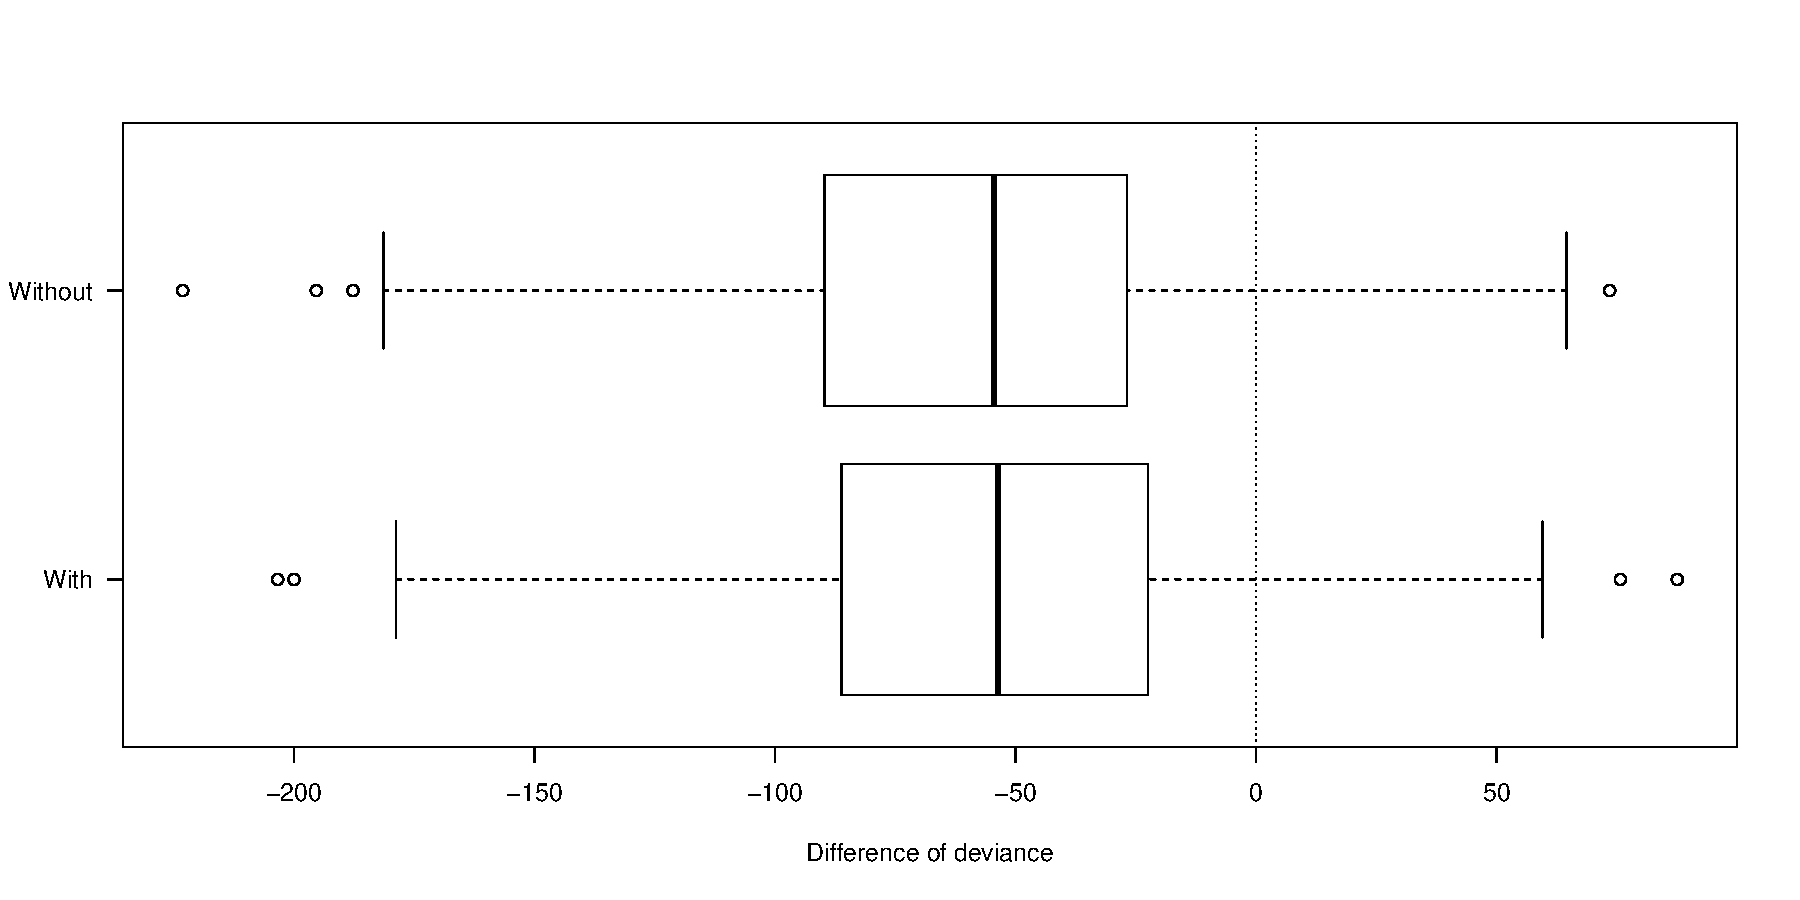
\includegraphics[scale=0.4]{deviances_simulation_correlated.pdf}
\end{figure}

For this scenario, as well, we see that the fixed intercept version has a higher optimal iteration number.
The median $\mstop$ is 50 with a fixed intercept, compared to a median of 19.5 for the changing intercept version.
Again this necessarily means that more variables are selected.
We see that the median deviance is very slightly better for the fixed intercept version, and with better extreme values, both minimum and maximum.
See Figure \ref{fig:simulation-correlated-deviances-boxplot} for a boxplot of the difference of deviance for the two versions.

Now consider the variable selection metrics.
We first look at the covariate vector $\bbeta$, which affects the initial level $y_0$.
The fixed intercept version is slightly better with regards to sensitivity, i.e., selecting informative variables, with a median of 0.200 versus a median of 0.143 for the changing intercept version.
This does come at a cost of a higher false discovery rate, with a median as high as 0.690, where the changing intercept version has a median of 0.500.
This means that we should expect that more than two in three 
In both versions, then, it is at least as likely to select a non-informative variable as an informative variable.
The specificity score is almost perfect in both cases, but again we note that the denominator $N$ is very large.

Look now at the ``clinical'' covariates, used in $\bgamma$ and related to the drift $\mu$.
The changing intercept version performs quite a lot worse here than the fixed intercept version.
It achieves a median sensitivity of 0.200, while the fixed intercept version achieves 0.700.
This does come at a cost of a lower specificity, with a median of 0.533 for the fixed intercept and 0.867 for the changing intercept.
Finally, the two versions actually have the same median false discovery rate, 0.500.
However, the mean of the fixed intercept is slightly higher, at 0.507, whereas the changing intercept version has a mean of 0.454.

In conclusion, while the fixed intercept version also here selects more true positive variables, it comes at a cost of selecting more false positives.
If we use the deviance to assess which one is best, then the fixed intercept version is the better one here as well.

\section{Discussion}
Based on the results in this simulation study, we conclude that it is better to use the fixed intercept version of the algorithm.
It has performed consistently, but only slightly better with regards to log-likelihood/deviance on out-of-sample data.
As we have discussed, the variable selection has trade offs.
The fixed intercept version selects more true positives, but it also selects more false positives.
It does seem to be worth it, in the end, since it achieves a better generalization error in the form of a lower difference of deviance.

\todo[inline]{Make clear that in the correlated case we are more close to real data, and here the differences are not huge!}